\documentclass{standalone}
\usepackage{ tikz }
\usepackage{ xparse }
\input{macros/all}

\begin{document}
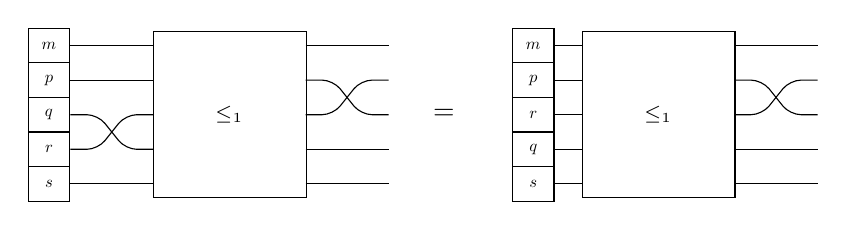
\begin{tikzpicture}[yscale=-1,x=1em,y=1.25em]

    \node[draw, minimum height = 1.25em, minimum width = 1.5em, anchor = east] at (0,0){\scalebox{0.6}{$m$}};
    \node[draw, minimum height = 1.25em, minimum width = 1.5em, anchor = east] at (0,1){\scalebox{0.6}{$p$}};
    \node[draw, minimum height = 1.25em, minimum width = 1.5em, anchor = east] at (0,2){\scalebox{0.6}{$q$}};
    \node[draw, minimum height = 1.25em, minimum width = 1.5em, anchor = east] at (0,3){\scalebox{0.6}{$r$}};
    \node[draw, minimum height = 1.25em, minimum width = 1.5em, anchor = east] at (0,4){\scalebox{0.6}{$s$}};

    \draw [rounded corners] (0,0) -- (3,0);
    \draw [rounded corners] (0,1) -- (3,1);
    \draw [rounded corners] (0,2) -- (1,2) -- (2,3) -- (3,3);
    \draw [rounded corners] (0,3) -- (1,3) -- (2,2) -- (3,2);
    \draw [rounded corners] (0,4) -- (3,4);

    \node[draw, minimum height = 6em, minimum width = 5.5em, anchor = west] at (3, 2){$\shuffle_{\leq_1}$};

    \draw [rounded corners] (8.5,0) -- (11.5,0);
    \draw [rounded corners] (8.5,1) -- (9.5,1) -- (10.5,2) -- (11.5,2);
    \draw [rounded corners] (8.5,2) -- (9.5,2) -- (10.5,1) -- (11.5,1);
    \draw [rounded corners] (8.5,3) -- (11.5,3);
    \draw [rounded corners] (8.5,4) -- (11.5,4);

    \node at (13.5,2){$=$};

    \node[draw, minimum height = 1.25em, minimum width = 1.5em, anchor = east] at (17.5,0){\scalebox{0.6}{$m$}};
    \node[draw, minimum height = 1.25em, minimum width = 1.5em, anchor = east] at (17.5,1){\scalebox{0.6}{$p$}};
    \node[draw, minimum height = 1.25em, minimum width = 1.5em, anchor = east] at (17.5,2){\scalebox{0.6}{$r$}};
    \node[draw, minimum height = 1.25em, minimum width = 1.5em, anchor = east] at (17.5,3){\scalebox{0.6}{$q$}};
    \node[draw, minimum height = 1.25em, minimum width = 1.5em, anchor = east] at (17.5,4){\scalebox{0.6}{$s$}};

    \draw [rounded corners] (17.5,0) -- (18.5,0);
    \draw [rounded corners] (17.5,1) -- (18.5,1);
    \draw [rounded corners] (17.5,2) -- (18.5,2);
    \draw [rounded corners] (17.5,3) -- (18.5,3);
    \draw [rounded corners] (17.5,4) -- (18.5,4);

    \node[draw, minimum height = 6em, minimum width = 5.5em, anchor = west] at (18.5, 2){$\shuffle_{\leq_1}$};

    \draw [rounded corners] (24,0) -- (27,0);
    \draw [rounded corners] (24,1) -- (25,1) -- (26,2) -- (27,2);
    \draw [rounded corners] (24,2) -- (25,2) -- (26,1) -- (27,1);
    \draw [rounded corners] (24,3) -- (27,3);
    \draw [rounded corners] (24,4) -- (27,4);

\end{tikzpicture}
\end{document}